% GNUPLOT: LaTeX picture with Postscript
\documentclass{minimal}
% Set font size
\makeatletter
\def\@ptsize{1}
\InputIfFileExists{size11.clo}{}{%
   \GenericError{(gnuplot) \space\space\space\@spaces}{%
      Gnuplot Error: File `size11.clo' not found! Could not set font size%
   }{See the gnuplot documentation for explanation.%
   }{For using a font size a file `size<fontsize>.clo' has to exist.
        Falling back ^^Jto default fontsize 10pt.}%
  \def\@ptsize{0}
  \input{size10.clo}%
}%
\makeatother
% Load packages
\usepackage{calc}
\usepackage{graphicx}
\usepackage{color}
\usepackage{transparent}
\makeatletter
% Select an appropriate default driver (from TeXLive graphics.cfg)
\begingroup
  \chardef\x=0 %
  % check pdfTeX
  \@ifundefined{pdfoutput}{}{%
    \ifcase\pdfoutput
    \else
      \chardef\x=1 %
    \fi
  }%
  % check VTeX
  \@ifundefined{OpMode}{}{%
    \chardef\x=2 %
  }%
\expandafter\endgroup
\ifcase\x
  % default case
  \PassOptionsToPackage{dvips}{geometry}
\or
  % pdfTeX is running in pdf mode
  \PassOptionsToPackage{pdftex}{geometry}
\else
  % VTeX is running
  \PassOptionsToPackage{vtex}{geometry}
\fi
\makeatother
% Set papersize
\usepackage[papersize={311.00bp,481.00bp},text={311.00bp,481.00bp}]{geometry}
% No page numbers and no paragraph indentation
\pagestyle{empty}
\setlength{\parindent}{0bp}%
% Load configuration file
\InputIfFileExists{gnuplot.cfg}{%
  \typeout{Using configuration file gnuplot.cfg}%
}{%
 \typeout{No configuration file gnuplot.cfg found.}%
}%
\renewcommand\familydefault{\sfdefault}\usepackage{cmbright}
\begin{document}
\begingroup
  \makeatletter
  \providecommand\color[2][]{%
    \GenericError{(gnuplot) \space\space\space\@spaces}{%
      Package color not loaded in conjunction with
      terminal option `colourtext'%
    }{See the gnuplot documentation for explanation.%
    }{Either use 'blacktext' in gnuplot or load the package
      color.sty in LaTeX.}%
    \renewcommand\color[2][]{}%
  }%
  \providecommand\includegraphics[2][]{%
    \GenericError{(gnuplot) \space\space\space\@spaces}{%
      Package graphicx or graphics not loaded%
    }{See the gnuplot documentation for explanation.%
    }{The gnuplot epslatex terminal needs graphicx.sty or graphics.sty.}%
    \renewcommand\includegraphics[2][]{}%
  }%
  \providecommand\rotatebox[2]{#2}%
  \@ifundefined{ifGPcolor}{%
    \newif\ifGPcolor
    \GPcolortrue
  }{}%
  \@ifundefined{ifGPblacktext}{%
    \newif\ifGPblacktext
    \GPblacktextfalse
  }{}%
  % define a \g@addto@macro without @ in the name:
  \let\gplgaddtomacro\g@addto@macro
  % define empty templates for all commands taking text:
  \gdef\gplbacktext{}%
  \gdef\gplfronttext{}%
  \makeatother
  \ifGPblacktext
    % no textcolor at all
    \def\colorrgb#1{}%
    \def\colorgray#1{}%
  \else
    % gray or color?
    \ifGPcolor
      \def\colorrgb#1{\color[rgb]{#1}}%
      \def\colorgray#1{\color[gray]{#1}}%
      \expandafter\def\csname LTw\endcsname{\color{white}}%
      \expandafter\def\csname LTb\endcsname{\color{black}}%
      \expandafter\def\csname LTa\endcsname{\color{black}}%
      \expandafter\def\csname LT0\endcsname{\color[rgb]{1,0,0}}%
      \expandafter\def\csname LT1\endcsname{\color[rgb]{0,1,0}}%
      \expandafter\def\csname LT2\endcsname{\color[rgb]{0,0,1}}%
      \expandafter\def\csname LT3\endcsname{\color[rgb]{1,0,1}}%
      \expandafter\def\csname LT4\endcsname{\color[rgb]{0,1,1}}%
      \expandafter\def\csname LT5\endcsname{\color[rgb]{1,1,0}}%
      \expandafter\def\csname LT6\endcsname{\color[rgb]{0,0,0}}%
      \expandafter\def\csname LT7\endcsname{\color[rgb]{1,0.3,0}}%
      \expandafter\def\csname LT8\endcsname{\color[rgb]{0.5,0.5,0.5}}%
    \else
      % gray
      \def\colorrgb#1{\color{black}}%
      \def\colorgray#1{\color[gray]{#1}}%
      \expandafter\def\csname LTw\endcsname{\color{white}}%
      \expandafter\def\csname LTb\endcsname{\color{black}}%
      \expandafter\def\csname LTa\endcsname{\color{black}}%
      \expandafter\def\csname LT0\endcsname{\color{black}}%
      \expandafter\def\csname LT1\endcsname{\color{black}}%
      \expandafter\def\csname LT2\endcsname{\color{black}}%
      \expandafter\def\csname LT3\endcsname{\color{black}}%
      \expandafter\def\csname LT4\endcsname{\color{black}}%
      \expandafter\def\csname LT5\endcsname{\color{black}}%
      \expandafter\def\csname LT6\endcsname{\color{black}}%
      \expandafter\def\csname LT7\endcsname{\color{black}}%
      \expandafter\def\csname LT8\endcsname{\color{black}}%
    \fi
  \fi
    \setlength{\unitlength}{0.0500bp}%
    \ifx\gptboxheight\undefined%
      \newlength{\gptboxheight}%
      \newlength{\gptboxwidth}%
      \newsavebox{\gptboxtext}%
    \fi%
    \setlength{\fboxrule}{0.5pt}%
    \setlength{\fboxsep}{1pt}%
\begin{picture}(6220.00,9620.00)%
    \gplgaddtomacro\gplbacktext{%
      \csname LTb\endcsname%%
      \put(736,7945){\makebox(0,0)[r]{\strut{}$20$}}%
      \csname LTb\endcsname%%
      \put(736,8369){\makebox(0,0)[r]{\strut{}$40$}}%
      \csname LTb\endcsname%%
      \put(736,8794){\makebox(0,0)[r]{\strut{}$60$}}%
      \csname LTb\endcsname%%
      \put(736,9218){\makebox(0,0)[r]{\strut{}$80$}}%
      \csname LTb\endcsname%%
      \put(838,7547){\makebox(0,0){\strut{}}}%
      \csname LTb\endcsname%%
      \put(2132,7547){\makebox(0,0){\strut{}}}%
      \csname LTb\endcsname%%
      \put(3427,7547){\makebox(0,0){\strut{}}}%
      \csname LTb\endcsname%%
      \put(4721,7547){\makebox(0,0){\strut{}}}%
      \csname LTb\endcsname%%
      \put(6015,7547){\makebox(0,0){\strut{}}}%
      \csname LTb\endcsname%%
      \put(62,9427){\makebox(0,0)[l]{\strut{}(a)}}%
      \csname LTb\endcsname%%
      \put(62,7599){\makebox(0,0)[l]{\strut{}(b)}}%
      \csname LTb\endcsname%%
      \put(62,5771){\makebox(0,0)[l]{\strut{}(c)}}%
      \csname LTb\endcsname%%
      \put(62,3944){\makebox(0,0)[l]{\strut{}(d)}}%
      \csname LTb\endcsname%%
      \put(62,2116){\makebox(0,0)[l]{\strut{}(e)}}%
    }%
    \gplgaddtomacro\gplfronttext{%
      \csname LTb\endcsname%%
      \put(346,8581){\rotatebox{-270}{\makebox(0,0){\strut{}MFPT $\mu/\tau$}}}%
      \csname LTb\endcsname%%
      \put(2208,9167){\makebox(0,0)[r]{\strut{}H $\rightarrow$ I$}}%
      \csname LTb\endcsname%%
      \put(2208,8981){\makebox(0,0)[r]{\strut{}I $\rightarrow$ H$}}%
      \csname LTb\endcsname%%
      \put(3302,9167){\makebox(0,0)[r]{\strut{}H $\rightarrow$ E$}}%
      \csname LTb\endcsname%%
      \put(3302,8981){\makebox(0,0)[r]{\strut{}E $\rightarrow$ H}}%
      \csname LTb\endcsname%%
      \put(4396,9167){\makebox(0,0)[r]{\strut{}I $\rightarrow$ E}}%
      \csname LTb\endcsname%%
      \put(4396,8981){\makebox(0,0)[r]{\strut{}E $\rightarrow$ I}}%
    }%
    \gplgaddtomacro\gplbacktext{%
      \csname LTb\endcsname%%
      \put(736,6200){\makebox(0,0)[r]{\strut{}$20$}}%
      \csname LTb\endcsname%%
      \put(736,6791){\makebox(0,0)[r]{\strut{}$40$}}%
      \csname LTb\endcsname%%
      \put(736,7381){\makebox(0,0)[r]{\strut{}$60$}}%
      \csname LTb\endcsname%%
      \put(838,5719){\makebox(0,0){\strut{}}}%
      \csname LTb\endcsname%%
      \put(2132,5719){\makebox(0,0){\strut{}}}%
      \csname LTb\endcsname%%
      \put(3427,5719){\makebox(0,0){\strut{}}}%
      \csname LTb\endcsname%%
      \put(4721,5719){\makebox(0,0){\strut{}}}%
      \csname LTb\endcsname%%
      \put(6015,5719){\makebox(0,0){\strut{}}}%
      \csname LTb\endcsname%%
      \put(62,9427){\makebox(0,0)[l]{\strut{}(a)}}%
      \csname LTb\endcsname%%
      \put(62,7599){\makebox(0,0)[l]{\strut{}(b)}}%
      \csname LTb\endcsname%%
      \put(62,5771){\makebox(0,0)[l]{\strut{}(c)}}%
      \csname LTb\endcsname%%
      \put(62,3944){\makebox(0,0)[l]{\strut{}(d)}}%
      \csname LTb\endcsname%%
      \put(62,2116){\makebox(0,0)[l]{\strut{}(e)}}%
    }%
    \gplgaddtomacro\gplfronttext{%
      \csname LTb\endcsname%%
      \put(366,6790){\rotatebox{-270}{\makebox(0,0){\strut{}STD $\sigma /\tau$}}}%
    }%
    \gplgaddtomacro\gplbacktext{%
      \csname LTb\endcsname%%
      \put(736,4077){\makebox(0,0)[r]{\strut{}$1.8$}}%
      \csname LTb\endcsname%%
      \put(736,4471){\makebox(0,0)[r]{\strut{}$2$}}%
      \csname LTb\endcsname%%
      \put(736,4865){\makebox(0,0)[r]{\strut{}$2.2$}}%
      \csname LTb\endcsname%%
      \put(736,5258){\makebox(0,0)[r]{\strut{}$2.4$}}%
      \csname LTb\endcsname%%
      \put(736,5652){\makebox(0,0)[r]{\strut{}$2.6$}}%
      \csname LTb\endcsname%%
      \put(838,3891){\makebox(0,0){\strut{}}}%
      \csname LTb\endcsname%%
      \put(2132,3891){\makebox(0,0){\strut{}}}%
      \csname LTb\endcsname%%
      \put(3427,3891){\makebox(0,0){\strut{}}}%
      \csname LTb\endcsname%%
      \put(4721,3891){\makebox(0,0){\strut{}}}%
      \csname LTb\endcsname%%
      \put(6015,3891){\makebox(0,0){\strut{}}}%
      \csname LTb\endcsname%%
      \put(62,9427){\makebox(0,0)[l]{\strut{}(a)}}%
      \csname LTb\endcsname%%
      \put(62,7599){\makebox(0,0)[l]{\strut{}(b)}}%
      \csname LTb\endcsname%%
      \put(62,5771){\makebox(0,0)[l]{\strut{}(c)}}%
      \csname LTb\endcsname%%
      \put(62,3944){\makebox(0,0)[l]{\strut{}(d)}}%
      \csname LTb\endcsname%%
      \put(62,2116){\makebox(0,0)[l]{\strut{}(e)}}%
    }%
    \gplgaddtomacro\gplfronttext{%
      \csname LTb\endcsname%%
      \put(356,4963){\rotatebox{-270}{\makebox(0,0){\strut{}skewness $\kappa$}}}%
    }%
    \gplgaddtomacro\gplbacktext{%
      \csname LTb\endcsname%%
      \put(736,2603){\makebox(0,0)[r]{\strut{}$0.05$}}%
      \csname LTb\endcsname%%
      \put(736,2958){\makebox(0,0)[r]{\strut{}$0.1$}}%
      \csname LTb\endcsname%%
      \put(736,3312){\makebox(0,0)[r]{\strut{}$0.15$}}%
      \csname LTb\endcsname%%
      \put(736,3667){\makebox(0,0)[r]{\strut{}$0.2$}}%
      \csname LTb\endcsname%%
      \put(838,2063){\makebox(0,0){\strut{}}}%
      \csname LTb\endcsname%%
      \put(2132,2063){\makebox(0,0){\strut{}}}%
      \csname LTb\endcsname%%
      \put(3427,2063){\makebox(0,0){\strut{}}}%
      \csname LTb\endcsname%%
      \put(4721,2063){\makebox(0,0){\strut{}}}%
      \csname LTb\endcsname%%
      \put(6015,2063){\makebox(0,0){\strut{}}}%
      \csname LTb\endcsname%%
      \put(62,9427){\makebox(0,0)[l]{\strut{}(a)}}%
      \csname LTb\endcsname%%
      \put(62,7599){\makebox(0,0)[l]{\strut{}(b)}}%
      \csname LTb\endcsname%%
      \put(62,5771){\makebox(0,0)[l]{\strut{}(c)}}%
      \csname LTb\endcsname%%
      \put(62,3944){\makebox(0,0)[l]{\strut{}(d)}}%
      \csname LTb\endcsname%%
      \put(62,2116){\makebox(0,0)[l]{\strut{}(e)}}%
    }%
    \gplgaddtomacro\gplfronttext{%
      \csname LTb\endcsname%%
      \put(142,3135){\rotatebox{-270}{\makebox(0,0){\strut{}occupation $\Pi$}}}%
      \csname LTb\endcsname%%
      \put(4059,3786){\makebox(0,0)[r]{\strut{}H}}%
      \csname LTb\endcsname%%
      \put(4745,3786){\makebox(0,0)[r]{\strut{}E}}%
      \csname LTb\endcsname%%
      \put(5431,3786){\makebox(0,0)[r]{\strut{}I}}%
    }%
    \gplgaddtomacro\gplbacktext{%
      \csname LTb\endcsname%%
      \put(736,735){\makebox(0,0)[r]{\strut{}$200$}}%
      \csname LTb\endcsname%%
      \put(736,1100){\makebox(0,0)[r]{\strut{}$500$}}%
      \csname LTb\endcsname%%
      \put(736,1464){\makebox(0,0)[r]{\strut{}$800$}}%
      \csname LTb\endcsname%%
      \put(736,1829){\makebox(0,0)[r]{\strut{}$1100$}}%
      \csname LTb\endcsname%%
      \put(838,428){\makebox(0,0){\strut{}$-10$}}%
      \csname LTb\endcsname%%
      \put(2132,428){\makebox(0,0){\strut{}$-5$}}%
      \csname LTb\endcsname%%
      \put(3427,428){\makebox(0,0){\strut{}$0$}}%
      \csname LTb\endcsname%%
      \put(4721,428){\makebox(0,0){\strut{}$5$}}%
      \csname LTb\endcsname%%
      \put(6015,428){\makebox(0,0){\strut{}$10$}}%
      \csname LTb\endcsname%%
      \put(62,9427){\makebox(0,0)[l]{\strut{}(a)}}%
      \csname LTb\endcsname%%
      \put(62,7599){\makebox(0,0)[l]{\strut{}(b)}}%
      \csname LTb\endcsname%%
      \put(62,5771){\makebox(0,0)[l]{\strut{}(c)}}%
      \csname LTb\endcsname%%
      \put(62,3944){\makebox(0,0)[l]{\strut{}(d)}}%
      \csname LTb\endcsname%%
      \put(62,2116){\makebox(0,0)[l]{\strut{}(e)}}%
    }%
    \gplgaddtomacro\gplfronttext{%
      \csname LTb\endcsname%%
      \put(142,1403){\rotatebox{-270}{\makebox(0,0){\strut{}$t_i /$ fs}}}%
      \csname LTb\endcsname%%
      \put(3426,149){\makebox(0,0){\strut{}$f~/ ( \epsilon / nm )$}}%
      \csname LTb\endcsname%%
      \put(4643,1974){\makebox(0,0)[r]{\strut{}$t_1$}}%
      \csname LTb\endcsname%%
      \put(5431,1974){\makebox(0,0)[r]{\strut{}$t_2$}}%
    }%
    \gplbacktext
    \put(0,0){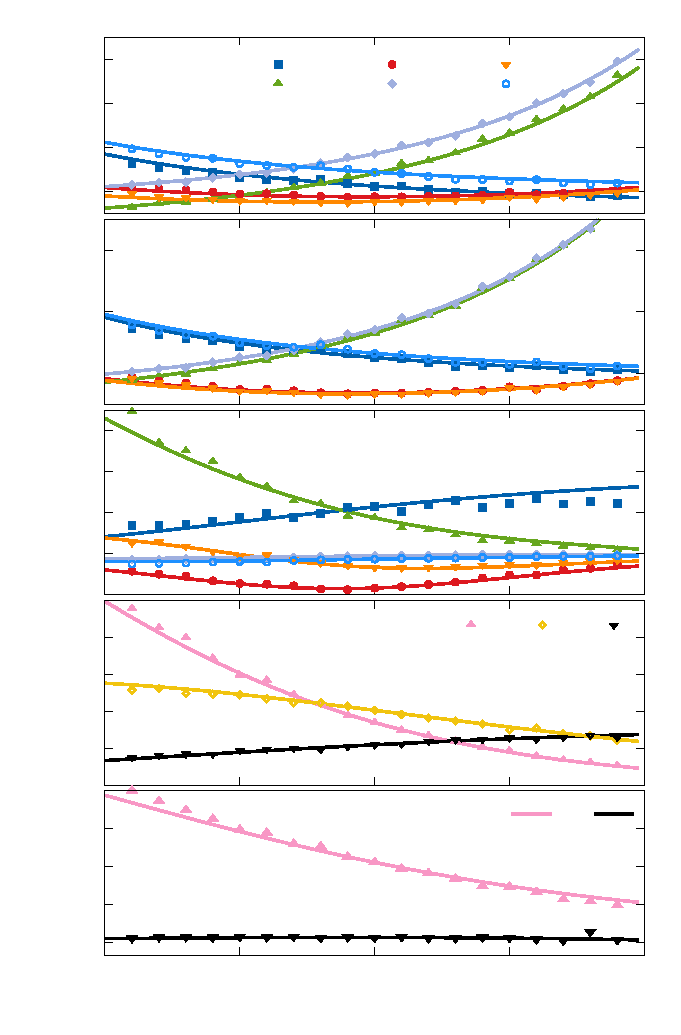
\includegraphics{mom_1001-inc}}%
    \gplfronttext
  \end{picture}%
\endgroup
\end{document}
